\chapter{Developer Documentation} % Developer guide
\label{ch:impl}

In this chapter, we are going to dive deep into the details of creating the log analyzer,
the architecture, and why the different parts of it were necessary, and how they all fit together.

To build and run the project as a developer, it is the same steps as in \ref{sec:installiation_guide}.
The user is expected to be able to add to the analyzer to match their different need and that is why
the roles of the developer and the user are very close to each other in the project.

As mentioned before, the log analyzer and the profiler are very tight, and to understand the analyzer's
design and its components, an overview of the profiler is needed. The next section covers this overview.
\newline
\begin{figure}[H]
	\centering
	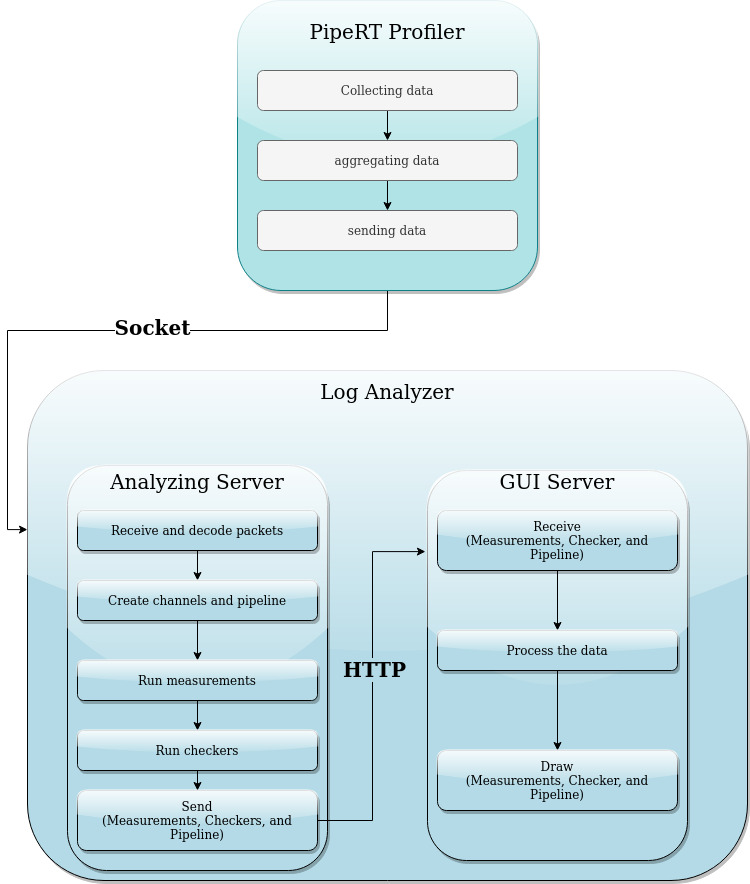
\includegraphics[width=0.9\textwidth,height=380px]{images/general_work_flow.jpg}
	\caption{General workflow}
	\label{fig:general_work_flow}
\end{figure}

\section{PipeRT Profiler} % Theorem-like items
The profiler is the utility in PipeRT responsible for profiling and monitoring functionality. It is a
sub-system to collect, aggregate, serialize, and send data to the log analyzer. The different configurations
of the profiler can be found at \ref{sec:server_side_config}.

The collection and aggregation of the profiler happen over different types of  events, there exist several
predefined events, however, the user can also add their events if needed. These different events are
the analyzer guideline for the channels' measurements and to understand the pipeline and measure it.

\subsection{Events}\label{sec:events}
The events are actions that happen to a packet in a channel. There are six predefined events, \textbf{Pushed},
\textbf{Retrieved}, \textbf{Execution Time}, \textbf{Fill Time}, \textbf{Read Time}, and \textbf{Dropped Packet}.

Since the profiler is supposed to aggregate these events, the \textit{log aggregator}, a helper utility in the profiler, is going to group these events
based on the event type, and these aggregated data will be sent to the log analyzer. Each aggregated event will have
a log count, and that is the number of logged events, and the time aggregation started, minimum time,
maximum time, and the average time that event took to complete.

\subsubsection{Pushed Event}\label{sec:pushed_event}
Time in packet's timeline when the packet is filled with data and pushed into the channel buffer.

\subsubsection{Retrieved Event}\label{sec:retrieved_event}
Time in packet's timeline when the packet is retrieved for processing.

\subsubsection{Execution Time Event}
Time spent by a scheduler thread servicing a channel callback.

\subsubsection{Fill Time Event}
Time spent between acquiring the packet and pushing it into the buffer

\subsubsection{Read Time Event}\label{sec:read_time_event}
Time spent between retrieving a packet and releasing it by the retriever

\subsubsection{Dropped Packet Event}
Packet was dropped because the buffer was full when the packet arrived.

\subsection{Sending Data} \label{sec:sending_data}
The profiler has a \textit{Sender Logger} auxiliary utility, which is responsible for serializing and sending
the data aggregated by the profiler. The sending part is the bridge of communication between the \textbf{PipeRT Profiler}
and the log analyzer so it was very important to consider the different possibilities before choosing the appropriate one.

Sending through sockets was the choice in sending and it is normal to use with such application, but the serialization
was not as clear of a choice, there are various ways to serialize the data, we are going to discuss four of them,
\textbf{binary sending}, \textbf{strings}, \textbf{XML} (Extensible Markup Language), and \textbf{protobuf} \cite{protobuf}.
Each one of them has its pros and cons.

Turn the data into a string is costing building the string and also any changes will mean changes in the
receiving side as well. The useful outtake of this option is the straightforward implementation.

Using XML as a format to communicate is a big burden on the performance and can lead to high memory usage,
that said XML is a very popular format and a go-to option based on the project.

Protobuf or protocol buffers from \textit{Google} is a work out of the box experience but will cost
extra maintenance in the long run and can be slow.

The final decision was using \textbf{binary sending}, despite that choosing this will lead to always make
sure that the \textbf{profiler} and \textbf{analyzer} are up to date with each other's sending and receiving
changes, the performance will be better compared to the other possibilities, and this performance
difference is an important key to minimize the delay hence having a better live analyzing which is the
main goal for the \textbf{log analyzer}.

\subsection{Packet serialization}\label{sec:packet_serialization}
The profiler sends packets of bytes, all the packets have the same structure, starts with \textit{DGRP}
as declaration of a new packet, null-terminated string of the receiver channel, 
\textit{SEND}, a null-terminated string of the sender channel, arbitrary number of aggregated data starts
with \textit{LOGA}, a null-terminated string of event's type, four bytes integer for \textit{log count}, 
four bytes integer for \textit{time passed in microseconds}, eight bytes double for \textit{minimum value}, 
eight bytes double for \textit{maximum value}, and eight bytes double for \textit{average value}.
\newline
\begin{figure}[H]
	\centering
	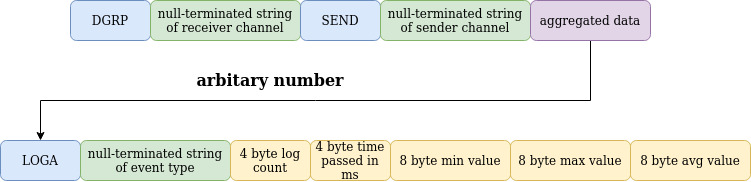
\includegraphics[width=1.0\textwidth,height=200px]{images/packet.jpg}
	\caption{Packet's structure}
	\label{fig:packet_structure}
\end{figure}

sending the packets is the last step in the profiler's workflow (\ref{fig:general_work_flow}) 
and from there, the log analyzer will start receiving and analyzing as we see in the following pages.

The log analyzer is separated into two main parts, as can be seen from \ref{fig:general_work_flow}.
In the next sections, details about these parts, their different components, and the connection between
them will be our topic.

\section{The Analyzing Server}
The first and the most vital part of the two, it is importance comes from its responsibility
to hold the logic of the analyzing, reading configuration, sending the data to the \textbf{GUI server}.
The coding of the \textbf{analyzing server} was done in \textit{python3} and the language choice was because
it is easy to use and fast to develop in which is suitable since it is expected from the user of the
analyzer to extend it to match their need.


The \textit{Front Controller Pattern} is the most used in the design of the \textbf{analyzing server},
and the \textit{Front Controller Pattern} is used to provide a centralized request handling 
mechanism so that all requests will be handled by a single handler which is very suitable to the various
checkers and measurements.

\textbf{AnalyzerServer} is the heart class of the \textbf{analyzing server} so it is the main controller
and responsible of starting and providing data for other controllers.

The first task for the \textbf{analyzing server} is to receive the packets from the profiler and decode it.

\subsection{Receiving and Decoding Packets}
Configuring the ip and port is crucial for successful receiving, the \textit{socket} library in python
is used to create the server and listen to the upcoming requests. The implementation of the server is
inside the \textbf{AnalyzerServer} class and upon receiving the packets the class is starting running the
other controllers.

The \textbf{PacketsManager} is the controller responsible for decoding the packets and distinguish them
by giving each of them different id number, it has two main methods, \textbf{add} to decode and add new packet
and \textbf{get\_latest\_packet} which is used as an input for another controller. The \textit{sigleton} 
desgin pattern was used to implement the \textbf{PacketsManager} as to have single instance of it 
everywhere in the code.
\newline
\begin{lstlisting}[language=python, label=PacketsManager, caption={puplic methods of PacketsManager},captionpos=b]
def add(self, packet):
	packet = PacketDecoder(packet).decode_packet()
	packet.set_id(self.__packets_count)
	packet.set_id_for_events()
	self.__latest_packet = packet
	self.__packets_count += 1

def get_latest_packet(self):
	return self.__latest_packet

def get_packet_count(self):
	return self.__packets_count

\end{lstlisting}

The packet is represented as \textbf{Packet} class, and it contains all the information that is sent
in the packet from the profiler (\ref{sec:packet_serialization}), and also has an id which is set by the
\textbf{PacketsManager}. The packet object has a method to set id for the events in it, and this method
is used by its controller as can be seen in \ref{PacketsManager}.

The event is also represented as \textbf{Event} class and contains the data for the type, log count, 
passed time, minimum value, maximum value, and average value. The packet can have more than one event
as mentioned in \ref{sec:events}, and that is represented as a list of events objects in the packet object.

The \textbf{PacketDecoder} is the utility responsible for decoding and insinuating the packet object. But
before going into details about how the decoding takes place, \textit{endianness} should be discussed first.

\textit{Endianness} is the order or sequence of bytes in computer memory. 
\textit{Endianness} is primarily expressed as big-endian (BE) or little-endian (LE). 
A big-endian system stores the most significant byte at the smallest memory address and 
the least significant byte at the largest. A little-endian system, in contrast, stores 
the least significant byte at the smallest address.
\newline
\begin{figure}[H]
	\centering
	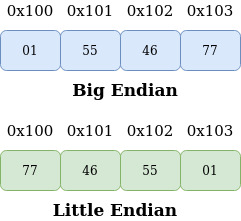
\includegraphics[width=0.9\textwidth,height=150px]{images/endianess.jpg}
	\caption{BE vs LE}
	\label{fig:be_vs_le}
\end{figure}
Since the packets comes in bytes (\ref{sec:sending_data}), the endianess of the bytes can form
an obstacle while decoding, python has some built-in utilities to overcome that and these utilities
were used in the decoding such as \textbf{decode} method for strings, \textbf{from\_bytes} method for integers,
and \textbf{unpack} method in \textbf{struct} data structure for double values.
\newline
\begin{lstlisting}[language=python, label=code:decoding, caption={decoding of a packet},captionpos=b]
def decode_packet(self):
	pos = 0
	if self.__check_for_correct_packet(self.__packet[pos:pos+4]):
		pos += 4
		receiver_channel_name, pos = self.__get_keyword(pos)
		sender_channel_name, pos = self.__get_keyword(pos)
		events = []
		correct_packet = self.__check_for_correct_packet(self.__packet[pos:pos+4])
		while not correct_packet and pos < len(self.__packet):
			event, pos = self.__get_event(pos)
			events.append(event)
		return Packet(receiver_channel_name, sender_channel_name, events)
	else:
		raise ValueError
\end{lstlisting}
Code \ref{code:decoding} is showing the \textbf{decode\_packet} method in the \textbf{PacketDecoder}
class, the algorithm is straightforward as it is following the bytes order as in figure \ref{fig:packet_structure}.
\newline
\begin{lstlisting}[language=python, label=code:decoding_methods, caption={helper methods in decoding},captionpos=b]
def __get_keyword(self, pos):
	keyword = b""
	while self.__packet[pos] != b"\x00":
		keyword += self.__packet[pos]
		pos += 1
	return keyword.decode("utf-8"), pos+1

def __get_int_val(self, pos):
	ret = b""
	for i in range(0, 4):
		ret += self.__packet[pos + i]
	pos += 4
	ret = int.from_bytes(ret, byteorder="big")
	return ret, pos

def __get_float_val(self, pos):
	ret = b""
	for i in range(0, 8):
		if byteorder == "little":
			ret += self.__packet[pos+(7-i)]
		else:
			ret += self.__packet[pos+i]
	[ret] = struct.unpack('d', ret)
	pos += 8
	return ret, pos
\end{lstlisting}

Code \ref{code:decoding_methods} shows the usage of the python decoding utilities mentioned before
and how they can be used for different types.

The next step after decoding is managing the channels and assign the events to the correct channels.

\subsection{Channels}
Every measurement and checker depends on channels, so that makes them the part holding much information
about the pipeline and the system performance. Each channel is represented by the \textbf{Channel} class,
and the controller for these channels is the \textbf{ChannelsManager} class.

The \textbf{Channel} class is responsible for representing the channel so it contains basic fields 
for name and events. The class is also storing the different checkers' flags and measurements. Each
is only storing events during the packet cycle as mentioned in \ref{sec:g_config}, the last packet id that
has been added to the channel is also stored as it is needed for measurements.

The \textbf{Channel} class is not only storing the measurements but also responsible for providing them
to send them to the \textbf{GUI server}, and different approaches were used to find a suitable logic.

\subsubsection{Checkers approach}
Checkers are sent at the end of every packet cycle, and as a first approach the measurements were sent
in the same way, but this leads to two issues, firstly, the \textbf{GUI server} has to update and redraw
the graphs too frequently that in a case when the profiler is sending very frequently that browser might
stop, secondly, not every measurement is worth of plotting, for example when having ten packet cycles with
the same measurement.

\subsubsection{Buffering approach}
We encountered two obstacles and in this approach, the intendant was to slow down the sending of the measurements
so that the browser can draw the graphs without overwhelming it. Instead of sending in every packet cycle,
the measurements are going to be stored in lists, and once the \textbf{AnalyzerServer} is requesting the measurements
the channel is going to send them, and empty the lists and this repeat every specific number of cycles. It is
implemented to be ten cycles for now.

\subsubsection{Buffering and RDB approach}
The buffering approach was successfully able to deal with the first obstacle, but that leaves the problem of
having unnecessary points in the graphs, to solve this issue, the \textit{Ramer–Douglas–Peucker algorithm} was introduced
in the implementation to reduce the number of plotted points. The \textit{Ramer–Douglas–Peucker algorithm}
also known as the \textbf{Douglas–Peucker algorithm} and \textbf{iterative end-point fit algorithm}, 
is an algorithm that decimates a curve composed of line segments to a similar curve with fewer points. 
It was one of the earliest successful algorithms developed for cartographic generalization. \cite{rdp}

The \textbf{Ramer–Douglas–Peucker algorithm} has it is own optimized library in python \cite{rdp_library},
and it was used to reduce the number of measurements in the graphs.
\newline
\begin{lstlisting}[language=python, label=code:rdp, caption={using rdp to reduce points},captionpos=b]
def reduce_points_n_extract_x_axis(points):
    minimized_points = rdp(points, epsilon=0.5)
    ret_points = [None] * 10
    for point in minimized_points:
        index = int((point[0] % 10) - 1)
        ret_points[index] = point[1]

    return ret_points
\end{lstlisting}

The \textbf{Ramer–Douglas–Peucker algorithm} calculations to reduce the points are based on epsilon's value,
and based on the choice of it, results can differ from each other on small scale, but for the analyzer use
\textbf{0.5} is general enough for the use case so it was implemented as can be seen from \ref{code:rdp}.
\newline
\begin{figure}[H]
	\centering
	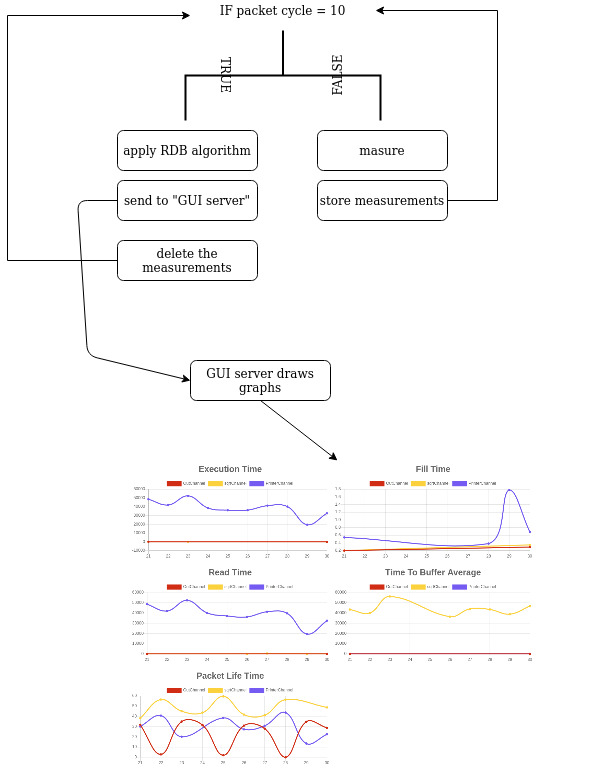
\includegraphics[width=1.0\textwidth,height=410px]{images/measurement_sending_cycle.jpg}
	\caption{Measurements sending mechanism}
	\label{fig:measurement cycle}
\end{figure}

The \textbf{ChannelsManager} is responsible for adding new channels, adding events for existent channels,
and creating the channels' map. It also contains a list of the channels in the pipeline 
and has a getter method to provide this list for the measurements or the checkers. Similar to the 
\textbf{PacketsManager}, the \textbf{ChannelsManager} is also implemented using a singleton design pattern.

In some packets, the sender is N/A channel which means that the channel has been fed data from a different
source other than the channels, for example, the first channel in the pipeline.

The \textbf{add\_packet} public method of it is used in the \textbf{AnalyzerServer}
and it is adding the receiver and the sender channels of the given packet. Adding the receiver is 
a matter of searching for the new channel name if it is not in the list, create a new channel
and add the packet's events to it, if it is already in the list add the events of 
the packet to the existent channel.
\newline
\begin{lstlisting}[language=python, label=code:add_packet, caption={add receiving channel},captionpos=b]
def add_packet(self, packet):
	receiver = packet.get_receiver()
	self.__add_reciever(receiver, packet.get_events(), packet.get_id())

	sender = packet.get_sender()
	pushed_events_count = packet.get_event_count(PACKET_PUSHED)
	self.__add_to_channels_map(receiver, sender, pushed_events_count)

def __add_reciever(self, receiver_channel, events, packet_id):
for channel in self.__channels:
	if channel.get_name() == receiver_channel:
		channel.add_events(events, self.__packets_cycle_threshold)
		channel.set_latest_packet_id(packet_id)
		should_add_reciever = False
		return

c = Channel(receiver_channel, events, packet_id)
self.__channels.append(c)
\end{lstlisting}

Adding the sender channel is taking into consideration the fact that the sender might be a N/A channel,
in order to determine if this a real N/A channel or the events in the packet did not need a sender, for 
example, \textbf{Read Time} (\ref{sec:read_time_event}) or \textbf{Retrieved} (\ref{sec:retrieved_event}) 
events do not require a sender so the packet
might have only these events so in this case the sender should not be added to the N/A channels.
The only event currently which requires a sender is the \textbf{Pushed} event (\ref{sec:pushed_event}).

Creating the channels' map is important to have the visualization of the pipeline and also, it is a vital
key for some measurements for example \textbf{time\_to\_buffer\_average} measurement (\ref{sec:time_to_buffer_average}).

The \textbf{\_\_add\_to\_channels\_map} method is holding the logic of adding to the channels' map,
it is checking if the sender is outside source, channel or there is no sender, and based on that it is adding
to the channels' map or not. If the sender is an outside source or a channel, a tuple containing both of them
will be added to the \textbf{\_\_channels\_map} list.
\newline
\begin{lstlisting}[language=python, caption={add to channels' map},captionpos=b]
def __add_to_channels_map(self, receiver, sender, pushed_event_cnt):
if not pushed_event_cnt:
	return
if sender == "N/A":
	sender = "External_" + receiver
	if sender not in self.__na_channels:
		self.__na_channels.append(sender)
else:
	channel_names = [c.get_name() for c in self.__channels]
	if sender not in channel_names:
		c = Channel(sender, [], -1)
		self.__channels.append(c)
sender_n_receiver = (sender, receiver)
if sender_n_receiver not in self.__channels_map:
	self.__channels_map.append(sender_n_receiver)
	self.__should_update_map = True	
\end{lstlisting}

The \textbf{ChannelsManager} has two public methods related to the channels' map, \textbf{get\_channels\_map}, 
and \textbf{should\_update\_map}. The \textbf{get\_channels\_map} method is returning two lists, the unique channels'
list and a list of tuples, each tuple represents a connection between two channels where the first element
is the sender and the second is the receiver. for example, in figure \ref{fig:pipeline_viz_home_page}, the unique
channels' list was equal to [OutChannel, sqrtChannel, PrinterChannel] and the list of connection was 
[(2,1),(1,0)]. The \textbf{should\_update\_map} method is implementing to send only in case a change happens
in the map and this preserves the resources taken to visualize the pipeline.
\newline
\begin{lstlisting}[language=python, caption={public methods for channels' map},captionpos=b]
def get_channels_map(self):
	channels_names = [c.get_name() for c in self.__channels]
	unique_channels = channels_names + self.__na_channels
	channels_dict = {c: i for i, c in enumerate(unique_channels)}
	connections = [(channels_dict[s], channels_dict[r]) for (s, r) in
				   self.__channels_map]
	return unique_channels, connections

def should_update_map(self):
	val = self.__should_update_map
	self.__should_update_map = False

	return val
\end{lstlisting}

The channel contains the measurements and the checkers' flags so to send these data
to the \textbf{GUI server}, two public methods were implemented in the \textbf{ChannelsManager}
and they are responsible for grouping the data into dictionaries so it can be sent through http 
post request in a json format.
\newline
\begin{lstlisting}[language=python, caption={data grouping methods},captionpos=b]
def get_channels_flags(self):
	return [{"name": channel.get_name(),
			"flags": channel.get_flags()}
			for channel in self.__channels]
	
def get_channels_measures(self):
	return [{"name": channel.get_name(),
			"measures": channel.get_all_measures()}
			for channel in self.__channels]
\end{lstlisting}
